\documentclass{article}
\usepackage{makeidx}
#\usepackage{fancyhdr}
#\pagestyle{fancy}
\usepackage[pdftex]{graphicx}

\begin{document}
\begin{center}
\title{Three dimensional coordinates into two dimensional coordinates transformation}\\
\author{Edward Gerhold}
\date{\today}
\maketitle

Version 0.1.5 (very drafty paper)\\

The formulas are correct. 
But the text itself is in the first stage.
And i have to learn \LaTeX{} for the first time.

}\\

June 25, 2015\\
\end{center}

\texbf{Remark} On a piece of paper you see three coordinate axis pointing into three
directions in space. In reality these vectors are two dimensional. Because
they point into three directions on the paper, and not into the real space.\\

[Picture of a 3-D coordinate system with ijk-vectors on the axis pointing
into three Directions]\\

In this document we will design a basis for the coordinate transformation. A
basis is multiplied with the value of the coordinate to move to the correct new point.\\
In the case of cosines and sines, we move left and right and up and down, to 
tell you directly, what happens, when we multiply the coordinates with the matrix.\\

The quick overview may move to the back as summarization.\\

\texbf{Quick overview}
\begin{enumerate}
\item Lay out the three base vectors around a circle and write down the angles $\varphi_n$.
\item Write down the base vectors $\vec{e}_n$ as $\cos \varphi$ and $\sin \varphi$ (two dimensional) with a unit length of $1$, or multiplied with $r_n \ne 1$.
\item Put the three base vectors $\vec{e}_n$ into a matrix \bigsymbol{A}. Programmers can directly code the two lines multiplication and forget the formal rest.
\item Iterate over your points and multiply each $(x,y,z)$ with the linear operator, the matrix \boldsymbol{A}, and put $(x',y')$ into your new set.
\end{enumerate}

\section{Definitions}

\texbf{Definition} Let $\varphi_n$ be the set of axis angles, one for each axis. The angles start
at the same place, at the number zero. You have to arrange the $x$, $y$, and
$z$ axes like on a piece of paper around the unit circle by giving them the
appropriate angles. All three angles start at the default at zero.\\

\begin{displaymath}
\varphi_n := \{\varphi_x, \varphi_y, \varphi_z\}
\end{displaymath}

\begin{example}
\texbf{Example}
The function rad converts degrees to radians, it´s useful for computer functions taking radians.
\begin{displaymath}
\text{rad } \phi := \frac{\pi}{180} \times \phi, \phi \element \Real
\end{displaymath}
Here is an example of three angles. The three axis have an angle of 120 degrees beetween each.
\begin{displaymath}
\varphi_x = \text{rad 210} ,
\varphi_y = \text{rad 330} ,
\varphi_z = \text{rad 90} 
\end{displaymath}
\end{example}

\texbf{Definition} Let $e_n$ be the set of three two dimensional unit base vectors, namely 
\vec{e}_x, $\vec{e}_y$ and $e_z$. Other names are $i$, $j$ or $k$ for example, like on the
picture of the coordinate system mentioned. The three vectors point into the three directions
of the three axis. On a piece of paper they are two dimensional, because they point into three
directions on the paper. The space being shown is what our brain completes, seeing three correct
axis. The three base vectors represent exactly one unit of each axis. \\

\begin{displaymath}
e_n := \{\vec{e}_x, \vec{e}_y, \vec{e}_z\}\\
\end{displaymath} 
 
This is the set of three unit vectors in set notation. To guess no numbers, it´s easier for us, 
for each vector, to go around the unit circle by the angles we already defined and to use cosine 
and sine for the correct $x$-distance and $y$-distance. For help, you should remember this parametrization 
of $x$ and $y$ from the unit circle.\\

\begin{displaymath}
\left(\begin{array}{1}x\\y\end{array}\right) = \left(\begin{array}{1}r \cos \varphi\\ r \sin \varphi\end{array}\right)\\
\end{displaymath}
\begin{displaymath}
(x,y) = (r \cos \varphi, r \sin \varphi)
\end{displaymath}

\begin{center}
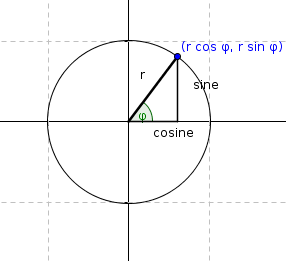
\includegraphics[scale=1]{unitcircle.png}
\end{center}

\texbf{Definition}

Modeling the three two dimensional base vectors with this information,
we get the following three two dimensional base vectors.\\

\begin{displaymath}
\vec{e}_x := (r_x\cos(\varphi_x), r_x\sin(\varphi_x) )^T = \left(\begin{array}{1}r_x\cos(\varphi_x)\\r_x\sin(\varphi_x) \end{array}\right)\\
\end{displaymath}
\begin{displaymath}
\vec{e}_y := (r_y\cos(\varphi_y), r_y\sin(\varphi_y) )^T = \left(\begin{array}{1}r_y\cos(\varphi_y)\\r_y\sin(\varphi_y) \end{array}\right)\\
\end{displaymath}
\begin{displaymath}
\vec{e}_z := (r_z\cos(\varphi_z), r_z\sin(\varphi_z) )^T = \left(\begin{array}{1}r_z\cos(\varphi_z)\\r_z\sin(\varphi_z) \end{array}\right)\\
\end{displaymath}

One for each component of $(x,y,z)$ By multiplying with, we move the 
points into the right pieces of direction. On the plane we use to point into three directions.\\

\begin{center}
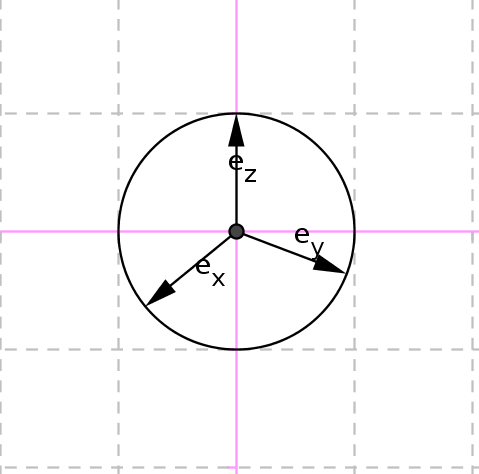
\includegraphics[scale=1]{unitvectors.png}
\end{center}

\texbf{Remark}.The values of $r_x, r_y$ and $r_z$ decide, how long one unit into each
direction is. To preserve affine graphical transformations all three
axes should have the same unit length, which can generally be enlarged
or made smaller than unit length. By default the resulting vector of the cos 
and sin Terms has unit length, if you don´t multiply with $r_x, r_y$ and $r_z$. \\

[here is a jump in the text, but it has to be rewritten anyways]\\

\emph{The other help we take} The other lemma we need is the theorem for 
multiplying with the orthogonal bases.
The sum of the basis multiplied with the coordinates is nothing
new. But Literature and lecture scripts just tell how to multiply
same dimensions, giving no clue about the easy 3-D to 2-D conversions.

\begin{displaymath}
\vec{v} = \displaystyle\sum_{n} \vec{e}_n\vec{x}_n
\end{displaymath}

Each $(x,y,z)$ coordinate has to be multiplied for the new $(x',y')$
with it´s corresponding term of the unit vectors in the matrix. That means,
to sum the products with $(x,y,z)$ and the cos terms up for $x'$ and to sum the products
of $(x,y,z)$ and the sin terms up for $y'$. This is the same as imagining walking left and
right with $\cos \varphi$ and up and down with $\sin \varphi$. Or mathematically adding positive or negative values.\\

\begin{displaymath}
\left(\begin{array}{1}x'\\y'\end{array}\right) = \left(\begin{array}{1}
xr_x\cos(\varphi_x) + yr_y\cos(\varphi_y) + zr_z\cos(\varphi_z)\\
xr_x\sin(\varphi_x) + yr_y\sin(\varphi_y) + zr_z\sin(\varphi_z)\end{array}\right)\\
\end{displaymath}

\texbf{Definition} Let A be the matrix containing the three two dimensional unit vectors in order, one each
column. You get a 2x3 matrix $\boldsymbol{A}: \Real^{3} \rightarrow \Real^{2}$.\footnote{A 2x3 Matrix, which i call the
Gerhold Projection Matrix to distinguish it from other matrices, making sure it contains the three two dimensional base vectors.
 for each of source coordinate components inside.} With the base vectors $\left(\begin{array}{1}\cos \varphi_n\\\sin \varphi_n\end{array}\right)$ in the three columns. 

\begin{displaymath}
\boldsymbol{A} := \left(
    \begin{array}{111}\vec{e}_x & \vec{e}_y & \vec{e}_z
    \end{array}\right)
    = \left(
    \begin{array}{111}
    r_x\cos(\varphi_x) & r_y\cos(\varphi_y) & r_z\cos(\varphi_z) \\
    r_x\sin(\varphi_x) & r_y\sin(\varphi_y) & r_z\sin(\varphi_z) \\
    \end{array}
\right)\\
\end{displaymath}

\section{Theorem}
\texbf{Theorem} \emph{(Fundamental Theorem of converting 3-D Points into 2-D Points)}:\\

If you multiply  \boldsymbol{A}, the matrix of the three two-dimensional unit vectors,
with the three-coordinate points $(x,y,z)$, the result is a two coordinate point, 
$(x',y')$. This point $(x',y')$ is the correct point on the two dimensional plane,
representing the point from the three dimensional coordinate system, we would like to display.\\

\begin{displaymath}
\boldsymbol{A}\left(\begin{array}{1}x\\y\\z\end{array}\right) = \left(\begin{array}{1}x'\\y'\end{array}\right)
\end{displaymath}

Applying the operator\footnote{The \emph{Gerholdian} operator is my favorite nickname for this matrix} performs the following operation\\

\begin{displaymath}
\boldsymbol{A}\left(\begin{array}{1}x\\y\\z\end{array}\right) = x\vec{e}_x + y\vec{e}_y + z\vec{e}_z\\
\end{displaymath}
\begin{displaymath}
= \left(\begin{array}{1}xr_x\cos(\varphi_x) + yr_y\cos(\varphi_y) + zr_z\cos(\varphi_z)\\
xr_x\sin(\varphi_x) + yr_y\sin(\varphi_y) + zr_z\sin(\varphi_z)\\
\end{array}\right) = \left(\begin{array}{1}x'\\y'\end{array}\right)
\end{displaymath}

\texbf{Proof}\\
\begin{displaymath}
\boldsymbol{A}\left(\begin{array}{1}x\\y\\z\end{array}\right) = x\vec{e}_x + y\vec{e}_y + z\vec{e}_z = \left(\begin{array}{1}x'\\y'\end{array}\right)
\end{displaymath}

\begin{displaymath}
\left(\begin{array}{1}x'\\y'\end{array}\right) = \left(\begin{array}{1}
xr_x\cos(\varphi_x) + yr_y\cos(\varphi_y) + zr_z\cos(\varphi_z)\\
xr_x\sin(\varphi_x) + yr_y\sin(\varphi_y) + zr_z\sin(\varphi_z)\end{array}\right)
\end{displaymath}\\

\texbf{Example}\\
\begin{example}
The following is an EcmaScript 6 (JavaScript) Arrow Function returning the new point. It is not optimized for speed. Means, to repeat the sin and cosine calls.\\
\texbf{Example for Programmers}
\mbox{ let projection = ([x,y,z]) => [x*r*Math.cos(xAxisAngle) + y*r*Math.cos(yAxisAngle) + z*r*Math.cos(zAxisAngle),x*r*Math.cos(xAxisAngle) + y*r*Math.sin(yAxisAngle) + z*r*Math.cos(zAxisAngle)]; }
\end{example}

\section{Corollary}

The theorem can be extended into more dimension to go down to any other dimension.
The generic case is known to linear algebra, i found it lately after beginning this
document and will include the information within the next versions.\\

\texbf{Corollary} \emph{(Converting any Dimensions down to less dimensions)}:\\

The theorem can be extended to more dimensions, for example can four two-dimensional
vectors represent a 4-D space on the 2-D plane. They get converted into the correct
 2-D points. For Example, if you use a 2x4 matrix and convert all points at each 
instance of $t$ you have a moving object into the direction of the fourth base vector. \\

\begin{displaymath}
\boldsymbol{A} := \left(
    \begin{array}{1111}\vec{e}_x & \vec{e}_y & \vec{e}_z & \vec{e}_t\end{array}\right)\\ = \left(
    \begin{array}{1111}
    r_x\cos(\varphi_x) & r_y\cos(\varphi_y) & r_z\cos(\varphi_z) & r_t\cos(\varphi_t)\\
    r_x\sin(\varphi_x) & r_y\sin(\varphi_y) & r_z\sin(\varphi_z) & r_t\sin(\varphi_t)\\
    \end{array}
\right)
\end{displaymath}


Here the basis is four times of two dimensions. A 2x4 matrix.\\

\begin{displaymath}
\boldsymbol{A}\left(\begin{array}{1}x\\y\\z\\t\end{array}\right) = \sum_{n} \vec{e}_n\vec{x}_n = \left(\begin{array}{1}x'\\y'\end{array}\right)$\\
\end{displaymath}

\texbf{Proof}:

\begin{displaymath}
\boldsymbol{A}\left(\begin{array}{1}x\\y\\z\\t\end{array}\right) = \left(\begin{array}{1}
xr_x\cos(\varphi_x) + yr_y\cos(\varphi_y) + zr_z\cos(\varphi_z) + zr_t\cos(\varphi_t)\\
xr_x\sin(\varphi_x) + yr_y\sin(\varphi_y) + zr_z\sin(\varphi_z)+ zr_t\sin(\varphi_t)\end{array}\right)\\
\end{displaymath}
\begin{displaymath}
= x\vec{e}_x + y\vec{e}_y + z\vec{e}_z + t\vec{e}_t = \sum_{n} \vec{e}_n\vec{x}_n = \left(\begin{array}{1}x'\\y'\end{array}\right)
\end{displaymath}

The same method can be used to convert any other number of dimensions to the $xy$-plane.
If you know the base vectors for the other dimensions you can convert down to other dimensions as well.\\

\texbf{References}:\\

\begin{thebibliography}
    \bibitem{[Corr09]} \textit{Michael Corral, Schoolcraft College},
		    Vector Calculus, http://mecmath.net,
		    
\end{thebibliography}


Will be updated after importing a few theorems, like the unit circle and the orthogonal basis vectors,
plus the generic mxn case of the "Abbildungsmatrix" i found lately after beginning this document.
Plus the free book containing the ijk-Picture which i used in mind to think about "how to project".\\

\makeindex
\printindex
\end{document}
